%\documentclass[12pt]{report}
%\documentclass[12pt]{extreport}
\documentclass[17pt]{article}
\usepackage{graphicx}
\usepackage{setspace}
\usepackage{amsmath,amssymb}
\usepackage{IEEEtrantools}
\usepackage{cancel}
\usepackage[font=small,labelfont=bf]{caption}

\usepackage{sectsty}

\sectionfont{\fontsize{12}{15}\selectfont}

\usepackage{geometry}
 \geometry{
 a4paper,
 total={170mm,264mm},
 left=20mm,
 top=10mm,
 }

\begin{document}

\begin{center}
	{\bf Formulario di elettromagnetismo (aggiornato al 14/05/2020})
\end{center}


\section{Forza elettrostatica}


\begin{itemize}
	\item Legge di Coulomb         
		\begin{itemize}
			\item Forma scalare $F = \frac{1}{4\pi\epsilon_0}\cdot\frac{qQ}{r^2}$
			\item Forma vettoriale $\vec{F} = \frac{1}{4\pi\epsilon_0}\cdot\frac{qQ}{r^2}\hat{r}$
		\end{itemize}			
	  
	\item Costante dielettrica del vuoto        $\epsilon_0 = 8.85\cdot 10^{-12}F/m$   (F = Farad)
\end{itemize}



\begin{figure}[th]
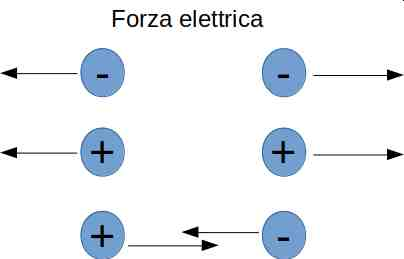
\includegraphics[width=6cm]{forzaElettrica.jpg}
\centering
\end{figure}






\subsection{Campo elettrico}

      
\begin{itemize}
	\item Forma scalare $E = \frac{1}{4\pi\epsilon_0}\cdot\frac{Q}{r^2}$ quindi $F = qE$
	\item Forma vettoriale $\vec{E} = \frac{1}{4\pi\epsilon_0}\cdot\frac{Q}{r^2}\hat{r}$ quindi $\vec{F} = q\vec{E}$
\end{itemize}			


\begin{figure}[th]
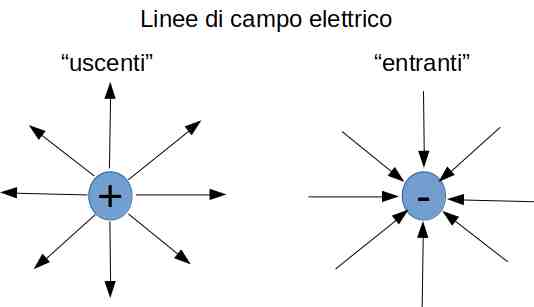
\includegraphics[width=8cm]{lineeCampoElettrico.jpg}
\centering
\end{figure}





\subsection{Forza elettrica e campo elettrico in un mezzo differente dal vuoto}
\emph{Le equazioni sono identiche} a quelle precedenti, soltanto che alla costante dielettrica del vuoto $\epsilon_0$ si sostituisce il prodotto $\epsilon_0\epsilon_r$, ove $\epsilon_r$ \'e la \emph{costante dielettrica relativa}, specifica del mezzo materiale ove l'interazione a distanza agisce.

\begin{itemize}
	\item Legge di Coulomb in un mezzo dielettrico       $F = \frac{1}{4\pi\epsilon_0\epsilon_r}\cdot\frac{qQ}{r^2}$ \\ $\epsilon_r$ costante dielettrica relativa (es. $\epsilon_{H_2O} = 81$)
	\item Forma scalare $E = \frac{1}{4\pi\epsilon_0\epsilon_r}\cdot\frac{Q}{r^2}$ quindi $F = qE$
	\item Forma vettoriale $\vec{E} = \frac{1}{4\pi\epsilon_0\epsilon_r}\cdot\frac{Q}{r^2}\hat{r}$ quindi $\vec{F} = q\vec{E}$
\end{itemize}

\section{Forza magnetica}

\begin{itemize}
	\item Forza magnetica tra due fili percorsi da corrente elettrica $i$ e $I$ rispettivamente: $F = \frac{\mu_0}{2\pi} \frac{iI}{d}$
	\begin{itemize}
		\item $\mu_0 = 4\pi\cdot 10^{-7}H/m$ costande diamagnetica del vuoto
		\item l = lunghezza dei due fili
		\item d = distanza tra i due fili
	\end{itemize}
\end{itemize}


\begin{figure}[th]
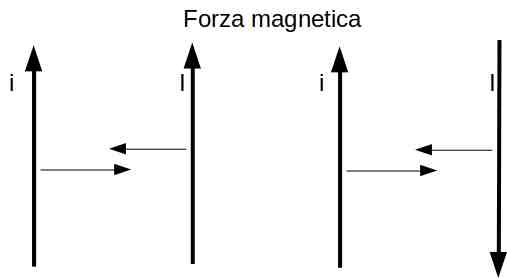
\includegraphics[width=8cm]{forzaMagnetica.jpg}
\centering
\end{figure}


\subsection{Campo magnetico}
Il campo magnetico \'e un \emph{campo vettoriale} $\vec{B}$

\begin{itemize}
	\item $B = \frac{\mu_0}{2\pi} \frac{I}{d}$ campo magnetico generato da un filo percorso da corrente $I$.
	\item $F = iBl$ Forza su un filo percorso da corrente $i$, dovuto alla presenza di un campo magnetico $B$ \emph{perpendicolare}.
	\item $\vec{F} = i\vec{B}\times\vec{l}$ Forma vettoriale della forza che un campo magnetico esercita su un filo di lunghezza $l$ percorso da corrente elettrica $i$.
	\item $\vec{F} = q\vec{v}\times\vec{B}$ Forma vettoriale della forza che un campo magnetico esercita su una carica in moto.
\end{itemize}

%\subsection{Forza magnetica e campo magnetico in un mezzo materiale}
\subsection{Forza magnetica e campo magnetico in un mezzo differente dal vuoto}

\emph{Le equazioni sono identiche} a quelle precedenti, soltanto che alla costante diamagnetica del vuoto$\mu_0$ si sostituisce il prodotto $\mu_0\mu_r$, ove $\mu_r$ \'e la \emph{costante diamagnetica relativa}, specifica del mezzo materiale ove l'interazione a distanza agisce.

%Le equazioni sono le stesse, soltanto che $\mu_0$ viene sostituita con $\mu_0\mu_r$, ove $\mu_r$ \'e la \emph{costante diamagnetica relativa}

\begin{itemize}
	\item Forza magnetica in un mezzo $F = \frac{\mu_0\mu_r}{2\pi} \frac{iI}{d}$.\\ $\mu_r$ \emph{costante diamagnetica relativa}
	\item $B = \frac{\mu_0\mu_r}{2\pi} \frac{I}{d}$
\end{itemize}

I materiali si distinguono in
\begin{itemize}
	\item diamagnetici $\mu_r < 0$
	\item paramagnetici $\mu_r > 0$
	\item ferromagnetici (calamite) 
\end{itemize}









\section{Distribuzione di carica }

\begin{itemize}
	\item $\lambda = \frac{\Delta Q}{\Delta l}$ distribuzione di carica lineare
	\item $\sigma = \frac{\Delta Q}{\Delta S}$ distribuzione di carica di superficie
	\item $\tau = \frac{\Delta Q}{\Delta V}$ distribuzione di carica di volume
\end{itemize}

\section{Campo elettrico indotto da una distribuzione piana di superficie}

Dal Teorema di Gauss applicato ad una superficie cilindrica con asse di simmetria perpendicolare alla superficie stessa il campo elettrico \'e
\begin{itemize}
	\item $E = \frac{\sigma}{2\epsilon_0}$ nel vuoto
	\item $E = \frac{\sigma}{2\epsilon_0\epsilon_r}$ se \'e presente un mezzo materiale differente dal vuoto.
\end{itemize}

La direzione di $\vec{E}$ \'e \emph{perpendicolare} alla superficie stessa e il verso \'e \emph{uscente} per distribuzione di carica positiva e \emph{entrante} per distribuzione di carica negativa


\section{Energia potenziale e potenziale elettrostatico}



\begin{itemize}
	\item Energia potenziale elettrostatica $U = \frac{1}{4\pi\epsilon_0}\frac{q_1q_2}{r}$ (si misura in Joule)
	\item Potenziale elettrostatico $V = \frac{1}{4\pi\epsilon_0}\frac{q}{r}$ (si misura in Volt)
	\item Differenza di potenziale dovuto a una carica puntiforme $\Delta V = V_A - V_B = \frac{q}{4\pi\epsilon_0}\cdot\left( \frac{1}{r_A} - \frac{1}{r_B} \right)$ 
\end{itemize}


\section{Condensatore}

Due lastre metalliche (armature) disposte molto vicine tra di loro. Funge da accumulatore di cariche: se si accumulano cariche positive in una delle due, sull'altra si accumulano cariche negative. In un condensatore a faccie piane e parallele si ha 

\begin{itemize}
	\item $E = \frac{\sigma}{\epsilon_0}$ tra le due lastre. Se \'e presente un mezzo, allora $E = \frac{\sigma}{\epsilon_0\epsilon_r}$
	\item $E = 0$ fuori dalle lastre
\end{itemize}


La grandezza che caratterizza un condensatore \'e la sua \emph{capacit\'a}

\begin{itemize}
	\item $C = \frac{Q}{\Delta V}\qquad$ Si esprime in \emph{Farad} (F)
\end{itemize}


Due condensatori possono esser collegati in \emph{serie} o in \emph{parallelo}

\begin{itemize}
	\item Serie $\frac{1}{C_{eq}} = \frac{1}{C_1} + \frac{1}{C_2}$
	\item Parallelo $C_{eq} = C_1 + C_2$
\end{itemize}

{\bf Densit\'a di energia} di volume accumulata da un condensatore (si considera un esperimento ideale in cui le cariche elettriche si fanno viaggiare da "infinitamente lontano" fino alle armature del condensatore stesso e, per ciascuna di esse, si calcola il lavoro necessario).

\begin{itemize}
	\item $u = \frac{1}{2} \epsilon_0E^2$
\end{itemize}

Questa espressione viene utilizzata, pi\'u in generale, come densit\'a di energia del campo elettrico ed ha applicazioni interessanti nelle onde elettromagnetiche.

\section{Resistenze elettriche}

\begin{itemize}
	\item Prima Legge di Ohm $V = Ri$
		\begin{itemize}
			\item V = Tensione, si esprime in Volt (V)
			\item R = Resistenza elettrica, si esprime in Ohm ($\Omega$)
			\item i = Intensit\'a di corrente elettrica, si esprime in Ampere (A)
		\end{itemize}
	\item Seconda Legge di Ohm $R=\rho\frac{l}{A}$
		\begin{itemize}
			\item R = Resistenza elettrica
			\item $\rho$ = Resistivit\'a, diversa per ogni materiale
			\item l = lunghezza
			\item A = Sezione
		\end{itemize}
	\item Serie $R_{eq} = R_1 + R_2$
	\item Parallelo $\frac{1}{R_{eq}} = \frac{1}{R_1} + \frac{1}{R_2}$
	\item Prima Legge di Kirchhoff: in un \emph{nodo} la somma delle correnti entranti \'e uguale alla somma delle correnti uscenti
	\item Seconda Legge di Kirchhoff: in una \emph{maglia} la somma delle cadute di potenziale \'e nulla
\end{itemize}



\section{Flusso di un campo}\label{sec:flusso}
Per semplicit\'a definiamo prima il flusso $\phi$ di un campo $\vec{E}$ \emph{costante} attraverso una superficie $\vec{S}$ \emph{piana}. 

Inoltre occorre definire il vettore superficie $\vec{S}$ come quel vettore la cui lunghezza \'e pari all'area $S$ della superficie e la cui direzione $\hat{n}$ \'e perpendicolare alla superficie stessa\footnote{In realt\'a questa definizione lascia una ambiguit\'a: il verso del vettore superficie non \'e stato definito. Non ha importanza quale sia questo verso, quel che conta \'e che, una volta deciso, si rimanga coerenti con tale decisione fino alla fine del problema.}. 

In queste condizioni il flusso \'e un prodotto scalare tra vettore campo $\vec{E}$ e vettore superficie $\vec{S}=S\hat{n}$. 

\begin{eqnarray}\label{eq:flusso}
	\phi(\vec{E}) = \vec{E}\cdot\vec{S}
\end{eqnarray}
	

\subsection{Flusso di un campo \emph{non} costante e/o superficie \emph{non} piana}

Occorre suddividere la superficie (che chiamiamo $\tau$) in N "pezzetti" $\Delta S_i$ (con $i = 1\dots N$) in ognuno dei quali il campo pu\'o approssimativamente essere considerato costante e la superficie pu\'o approssimativamente considerarsi piana. Per ciascuno di questi "pezzetti" (pezzetto i-esimo) si pu\'o applicare la definizione di flusso secondo l'equazione precedente ($\phi_i(\vec{E}) = \vec{E}_i\cdot\Delta\vec{S}_i$).

(Il limite del) La somma di tutti questi flussi \emph{infinitesimi} costituisce il flusso totale, si tratta di un integrale definito, e si scrive

\begin{eqnarray}
	\phi(\vec{E}) = \int_{\tau}\vec{E}\cdot d\vec{S} 
\end{eqnarray}

%\footnote{Pi\'u precisamente il \emph{limite} per $\Delta S\rightarrow 0$ di questa somma \'e il flusso $\phi(\vec{E}$)}.

\subsection{Flusso del campo elettrico (Prima Legge di Maxwell)}
Noto come \emph{Teorema di Gauss}.\\
Il flusso del campo elettrico attraverso una superficie \emph{chiusa} (quindi \emph{non} piana!) \'e pari alla somma delle cariche interne alla superficie diviso per la costante dielettrica $\epsilon_0$\footnote{Ovviamente, se il sistema \'e immerso in un mezzo dielettrico, allora $\epsilon_0$ va sostituito con il prodotto $\epsilon_0\epsilon_r$}


\begin{eqnarray}
	\phi(\vec{E}) = \int_{\tau}\vec{E}\cdot d\vec{S} = \frac{Q_{in}}{\epsilon_0}
\end{eqnarray}

\subsection{Flusso del campo magnetico (Terza Legge di Maxwell)}

Il flusso del campo magnetico attraverso una superficie \emph{chiusa} (quindi \emph{non} piana!) \'e sempre nullo!

\begin{eqnarray}
	\phi(\vec{B}) = \int_{\tau}\vec{B}\cdot d\vec{S} = 0
\end{eqnarray}


\section{Circuitazione}

Come il flusso, cos\'i anche la circuitazione si applica sia al campo elettrico $\vec{E}$ che al campo magnetico $\vec{B}$. \\
Se il campo \'e costante e il tratto $l$ ove si esegue la circuitazione \'e un rettilino allora, in anaolgia con quanto fatto con il flusso, si pu\'o eseguire il prodotto scalare
\begin{eqnarray}
	\vec{E}\cdot \Delta\vec{l}
\end{eqnarray}
il cui risultato, per definizione di prodotto scalare, \'e un numero. Si considera ora un circuito chiuso $\gamma$ (quindi \emph{non} rettilineo), lo si divide in tanti intervalli "infinitesimi" $\Delta l_i$, in modo tale che ciascuno di essi possa esser considerato lineare e il campo possa essere considerato costante. Per ciascuno di essi si pu\'o eseguire il suddetto prodotto scalare 
\begin{eqnarray}
	C_i = \vec{E}_i\cdot\Delta \vec{l}_i
\end{eqnarray}
 

La circuitazione \'e la somma di questi $C_i$ su un circuito \emph{chiuso} e si esprime
\begin{itemize}
	\item $ C(\vec{E}) = \sum_i  \vec{E}_i\cdot\Delta \vec{l}_i$
\end{itemize}

Nel limite che questi elementi $\Delta s_i$ diventino infinitamente piccoli, la suddetta sommatoria diventa un integrale e viene scritta cos\'i
$$
C(\vec{E}) = \oint_{\gamma} \vec{E}\cdot d\vec{l}
$$


\subsection{Circuitazione del campo elettrico (Terza Legge di Maxwell)}

Dato un circuito $\gamma$ \emph{chiuso}, si dimostra che la circuitazione del campo elettrico \'e pari a meno la variazione nel tempo del flusso del campo magnetico (Legge di Faray-Neumnann)


\begin{eqnarray}
	C(E)= \int_{\gamma}\vec{E}\cdot d\vec{l} = -\frac{\Delta \phi(\vec{B})}{\Delta t}
\end{eqnarray}

\subsection{Circuitazione del campo magnetico (Quarta Legge di Maxwell)}

Dato un circuito $\gamma$ \emph{chiuso}, si dimostra che la circuitazione del campo magnetico \'e proporzionale alla \emph{somma delle correnti concatenate}

\begin{eqnarray}
	C(B)= \int_{\gamma}\vec{B}\cdot d\vec{l} = \mu_0 i
\end{eqnarray}



\section{Campo magnetico generato da un solenoide di n spire}
\begin{itemize}
	\item $B = \mu_0 ni$
\end{itemize}






\section{Onde elettromagnetiche}

Il dipolo elettrico \'e costituito da due cariche di uguale intensit\'a ma opposte tra loro e disposte molto vicine l'una rispetto all'altra. Il dipolo \'e un sistema elettricamente carico ma che genera un campo elettrico \emph{non nullo} intorno a se. La molecola dell'acqua \'e un esempio di dipolo elettrico. Quando un dipolo elettrico oscilla, genera intorno a se una \emph{perturbazione del campo elettromagnetico che si propaga nello spazio e nel tempo} ad una velocit\'a $c = 3\cdot 10^{8}m/s$. Tale perturbazione si chiama \emph{onda elettromagnetica}.

\begin{figure}[th]
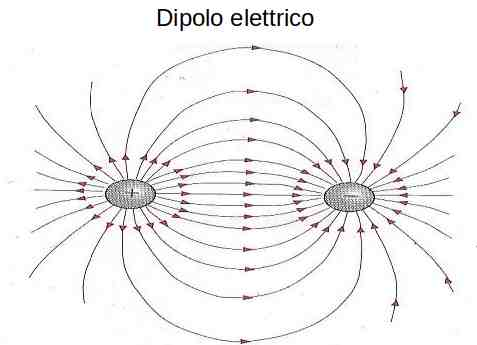
\includegraphics[width=8cm]{dipoloElettrico.jpg}
\centering
\end{figure}

\end{document}